% Options for packages loaded elsewhere
\PassOptionsToPackage{unicode}{hyperref}
\PassOptionsToPackage{hyphens}{url}
%
\documentclass[
  spanish,
  ignorenonframetext,
]{beamer}
\usepackage{pgfpages}
\setbeamertemplate{caption}[numbered]
\setbeamertemplate{caption label separator}{: }
\setbeamercolor{caption name}{fg=normal text.fg}
\beamertemplatenavigationsymbolsempty
% Prevent slide breaks in the middle of a paragraph
\widowpenalties 1 10000
\raggedbottom
\setbeamertemplate{part page}{
  \centering
  \begin{beamercolorbox}[sep=16pt,center]{part title}
    \usebeamerfont{part title}\insertpart\par
  \end{beamercolorbox}
}
\setbeamertemplate{section page}{
  \centering
  \begin{beamercolorbox}[sep=12pt,center]{part title}
    \usebeamerfont{section title}\insertsection\par
  \end{beamercolorbox}
}
\setbeamertemplate{subsection page}{
  \centering
  \begin{beamercolorbox}[sep=8pt,center]{part title}
    \usebeamerfont{subsection title}\insertsubsection\par
  \end{beamercolorbox}
}
\AtBeginPart{
  \frame{\partpage}
}
\AtBeginSection{
  \ifbibliography
  \else
    \frame{\sectionpage}
  \fi
}
\AtBeginSubsection{
  \frame{\subsectionpage}
}
\usepackage{lmodern}
\usepackage{amssymb,amsmath}
\usepackage{ifxetex,ifluatex}
\ifnum 0\ifxetex 1\fi\ifluatex 1\fi=0 % if pdftex
  \usepackage[T1]{fontenc}
  \usepackage[utf8]{inputenc}
  \usepackage{textcomp} % provide euro and other symbols
\else % if luatex or xetex
  \usepackage{unicode-math}
  \defaultfontfeatures{Scale=MatchLowercase}
  \defaultfontfeatures[\rmfamily]{Ligatures=TeX,Scale=1}
\fi
\usetheme[]{Berlin}
\usecolortheme{beaver}
% Use upquote if available, for straight quotes in verbatim environments
\IfFileExists{upquote.sty}{\usepackage{upquote}}{}
\IfFileExists{microtype.sty}{% use microtype if available
  \usepackage[]{microtype}
  \UseMicrotypeSet[protrusion]{basicmath} % disable protrusion for tt fonts
}{}
\makeatletter
\@ifundefined{KOMAClassName}{% if non-KOMA class
  \IfFileExists{parskip.sty}{%
    \usepackage{parskip}
  }{% else
    \setlength{\parindent}{0pt}
    \setlength{\parskip}{6pt plus 2pt minus 1pt}}
}{% if KOMA class
  \KOMAoptions{parskip=half}}
\makeatother
\usepackage{xcolor}
\IfFileExists{xurl.sty}{\usepackage{xurl}}{} % add URL line breaks if available
\IfFileExists{bookmark.sty}{\usepackage{bookmark}}{\usepackage{hyperref}}
\hypersetup{
  pdflang={es},
  hidelinks,
  pdfcreator={LaTeX via pandoc}}
\urlstyle{same} % disable monospaced font for URLs
\newif\ifbibliography
\usepackage{color}
\usepackage{fancyvrb}
\newcommand{\VerbBar}{|}
\newcommand{\VERB}{\Verb[commandchars=\\\{\}]}
\DefineVerbatimEnvironment{Highlighting}{Verbatim}{commandchars=\\\{\}}
% Add ',fontsize=\small' for more characters per line
\newenvironment{Shaded}{}{}
\newcommand{\AlertTok}[1]{\textcolor[rgb]{1.00,0.00,0.00}{\textbf{#1}}}
\newcommand{\AnnotationTok}[1]{\textcolor[rgb]{0.38,0.63,0.69}{\textbf{\textit{#1}}}}
\newcommand{\AttributeTok}[1]{\textcolor[rgb]{0.49,0.56,0.16}{#1}}
\newcommand{\BaseNTok}[1]{\textcolor[rgb]{0.25,0.63,0.44}{#1}}
\newcommand{\BuiltInTok}[1]{#1}
\newcommand{\CharTok}[1]{\textcolor[rgb]{0.25,0.44,0.63}{#1}}
\newcommand{\CommentTok}[1]{\textcolor[rgb]{0.38,0.63,0.69}{\textit{#1}}}
\newcommand{\CommentVarTok}[1]{\textcolor[rgb]{0.38,0.63,0.69}{\textbf{\textit{#1}}}}
\newcommand{\ConstantTok}[1]{\textcolor[rgb]{0.53,0.00,0.00}{#1}}
\newcommand{\ControlFlowTok}[1]{\textcolor[rgb]{0.00,0.44,0.13}{\textbf{#1}}}
\newcommand{\DataTypeTok}[1]{\textcolor[rgb]{0.56,0.13,0.00}{#1}}
\newcommand{\DecValTok}[1]{\textcolor[rgb]{0.25,0.63,0.44}{#1}}
\newcommand{\DocumentationTok}[1]{\textcolor[rgb]{0.73,0.13,0.13}{\textit{#1}}}
\newcommand{\ErrorTok}[1]{\textcolor[rgb]{1.00,0.00,0.00}{\textbf{#1}}}
\newcommand{\ExtensionTok}[1]{#1}
\newcommand{\FloatTok}[1]{\textcolor[rgb]{0.25,0.63,0.44}{#1}}
\newcommand{\FunctionTok}[1]{\textcolor[rgb]{0.02,0.16,0.49}{#1}}
\newcommand{\ImportTok}[1]{#1}
\newcommand{\InformationTok}[1]{\textcolor[rgb]{0.38,0.63,0.69}{\textbf{\textit{#1}}}}
\newcommand{\KeywordTok}[1]{\textcolor[rgb]{0.00,0.44,0.13}{\textbf{#1}}}
\newcommand{\NormalTok}[1]{#1}
\newcommand{\OperatorTok}[1]{\textcolor[rgb]{0.40,0.40,0.40}{#1}}
\newcommand{\OtherTok}[1]{\textcolor[rgb]{0.00,0.44,0.13}{#1}}
\newcommand{\PreprocessorTok}[1]{\textcolor[rgb]{0.74,0.48,0.00}{#1}}
\newcommand{\RegionMarkerTok}[1]{#1}
\newcommand{\SpecialCharTok}[1]{\textcolor[rgb]{0.25,0.44,0.63}{#1}}
\newcommand{\SpecialStringTok}[1]{\textcolor[rgb]{0.73,0.40,0.53}{#1}}
\newcommand{\StringTok}[1]{\textcolor[rgb]{0.25,0.44,0.63}{#1}}
\newcommand{\VariableTok}[1]{\textcolor[rgb]{0.10,0.09,0.49}{#1}}
\newcommand{\VerbatimStringTok}[1]{\textcolor[rgb]{0.25,0.44,0.63}{#1}}
\newcommand{\WarningTok}[1]{\textcolor[rgb]{0.38,0.63,0.69}{\textbf{\textit{#1}}}}
\usepackage{graphicx}
\makeatletter
\def\maxwidth{\ifdim\Gin@nat@width>\linewidth\linewidth\else\Gin@nat@width\fi}
\def\maxheight{\ifdim\Gin@nat@height>\textheight\textheight\else\Gin@nat@height\fi}
\makeatother
% Scale images if necessary, so that they will not overflow the page
% margins by default, and it is still possible to overwrite the defaults
% using explicit options in \includegraphics[width, height, ...]{}
\setkeys{Gin}{width=\maxwidth,height=\maxheight,keepaspectratio}
% Set default figure placement to htbp
\makeatletter
\def\fps@figure{htbp}
\makeatother
\setlength{\emergencystretch}{3em} % prevent overfull lines
\providecommand{\tightlist}{%
  \setlength{\itemsep}{0pt}\setlength{\parskip}{0pt}}
\setcounter{secnumdepth}{-\maxdimen} % remove section numbering
\usepackage[utf8]{inputenc}
\ifxetex
  % Load polyglossia as late as possible: uses bidi with RTL langages (e.g. Hebrew, Arabic)
  \usepackage{polyglossia}
  \setmainlanguage[]{spanish}
\else
  \usepackage[shorthands=off,main=spanish]{babel}
\fi

\author{}
\date{}

\begin{document}

\begin{frame}[fragile]
\begin{Shaded}
\begin{Highlighting}[]
\FunctionTok{Campus}\KeywordTok{:}\AttributeTok{ Ciudad Universitaria}
\FunctionTok{Facultad}\KeywordTok{:}\AttributeTok{ Ingeniería}
\FunctionTok{Materia }\KeywordTok{:}\AttributeTok{ Inteligencia Artificial}
\FunctionTok{Semestre}\KeywordTok{:}\AttributeTok{ 2022{-}2}
\FunctionTok{Equipo}\KeywordTok{:}\AttributeTok{ }\DecValTok{1}
\FunctionTok{Clave}\KeywordTok{:}\AttributeTok{ }\DecValTok{0406}
\FunctionTok{Participantes}\KeywordTok{:}\AttributeTok{ }
\KeywordTok{{-}}\AttributeTok{ Barrera Peña Víctor Miguel}
\KeywordTok{{-}}\AttributeTok{ Espino De Horta Joaquín Gustavo}
\AttributeTok{    }
\FunctionTok{Profesor}\KeywordTok{:}\AttributeTok{ Dr. Ismael Everardo Barcenas Patiño}
\FunctionTok{Título }\KeywordTok{:}\AttributeTok{ Proyecto 4}
\FunctionTok{Subtítulo }\KeywordTok{:}\AttributeTok{ Clasificador de imagenes}
\FunctionTok{Fecha entrega}\KeywordTok{:}\AttributeTok{ 26/05/2022}
\end{Highlighting}
\end{Shaded}

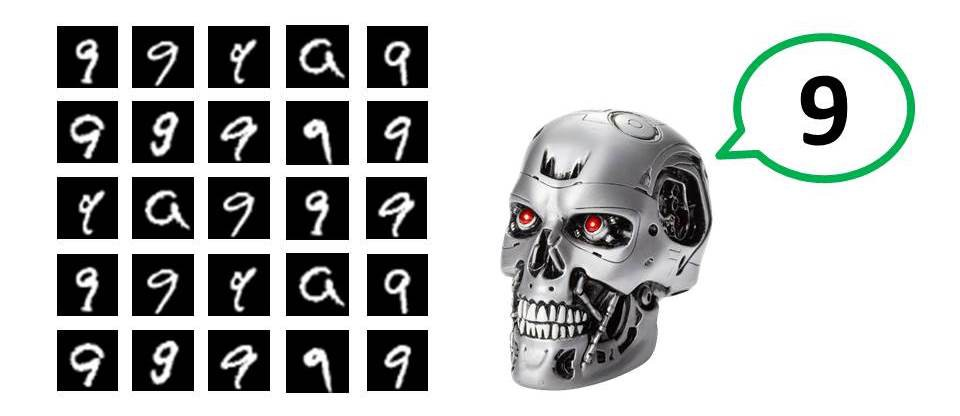
\includegraphics[width=1.1\textwidth,height=\textheight]{img/README/portada.jpeg}

\pagebreak
\end{frame}

\begin{frame}{Capítulo 0 Estructura del repositorio}
\protect\hypertarget{capuxedtulo-0-estructura-del-repositorio}{}
\begin{figure}
\centering
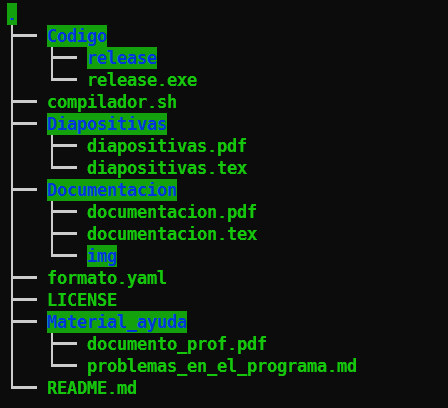
\includegraphics{img/README/Screenshot_1.png}
\caption{Tabla de contenido del repositorio}
\end{figure}
\end{frame}

\begin{frame}{Capítulo 1 Introducción}
\protect\hypertarget{capuxedtulo-1-introducciuxf3n}{}
La clasificación de imágenes es un concepto bastante viejo, aunque no
pareciese así, digamos que tiene entre 50 y 60 (1960-1970) años la
primera vez que se utilizó una tecnología así, sólo que esa vez era más
primitiva, por varias razones, tenemos que pensar que en ese tiempo las
computadoras, todavía trabajaban con grandes computadoras que ocupaban
un cuarto, todavía no estaba la teoría para la creación

Pero ¿Qué era lo que realmente realizaba? La clasificación entre hombres
y mujeres. ¿Cómo lo realizaba? Primero quiero que te imágenes señoritas
vestidas con pelo más abultado que el de los caballeros, sólo se usaba
foto de los hombros hacia arriba, se usaban sensores sensibles a la luz,
para poder pasar fotografías analógicas a digital, posterior a ello este
daba un mensaje diciendo si era hombre o mujer, es un excelente
antecedente de clasificación de imágenes.

Empezamos con el siguiente investigador que se acerca más a lo que es mi
proyecto, ya que el uso celdas foto sensibles para pasar trazos a
letras, esto es para digitalizarlos, pero además le enseño a hablar, es
decir pronunciar las palabras en el lenguaje inglés, resumiendo esto, el
hizo una clasificación de letras y además una red neural para que
pudieran hablar.

\begin{figure}
\centering
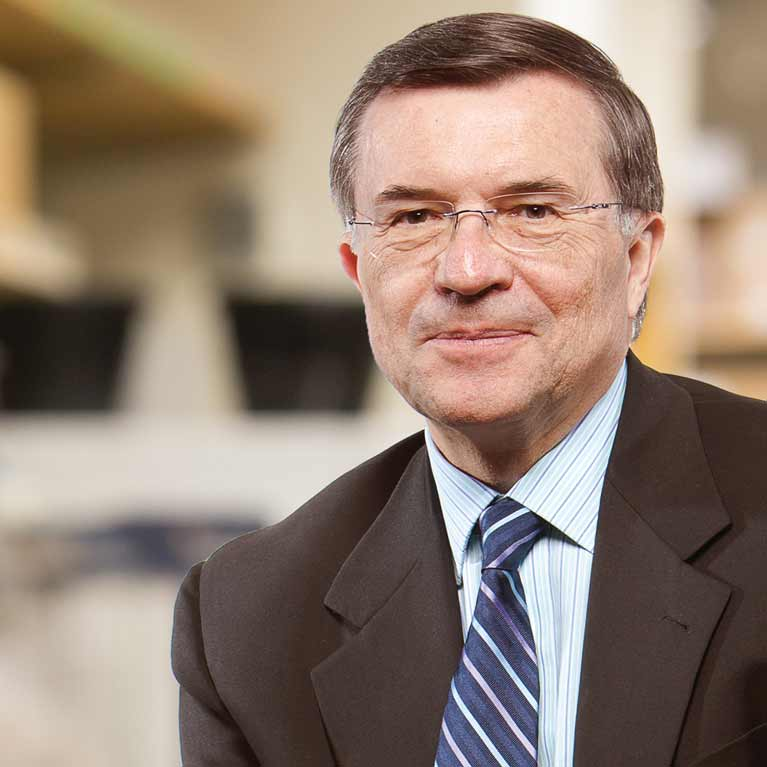
\includegraphics[width=0.3\textwidth,height=\textheight]{img/README/terrence.jpg}
\caption{Phd. Terrence Sejnowski}
\end{figure}

Retomando lo hecho por los antes mencionados, implementó, pero ahora
usando computadoras modernas, y con mucha mayor potencia, que aquellos
tiempos, y ahora todo siendo digital, mediante lenguajes de programación
y probabilidad, en lugar de redes neuronales como en 1986.
\end{frame}

\begin{frame}{Definición del problema}
\protect\hypertarget{definiciuxf3n-del-problema}{}
\end{frame}

\begin{frame}{Solución}
\protect\hypertarget{soluciuxf3n}{}
\begin{block}{Pseudocódigo}
\protect\hypertarget{pseudocuxf3digo}{}
\end{block}

\begin{block}{Explicación}
\protect\hypertarget{explicaciuxf3n}{}
\end{block}
\end{frame}

\begin{frame}{Experimentos}
\protect\hypertarget{experimentos}{}
\begin{block}{Baja dificultad}
\protect\hypertarget{baja-dificultad}{}
\begin{block}{Problema 1}
\protect\hypertarget{problema-1}{}
\end{block}

\begin{block}{Problema 2}
\protect\hypertarget{problema-2}{}
\end{block}

\begin{block}{Problema 3}
\protect\hypertarget{problema-3}{}
\end{block}
\end{block}

\begin{block}{Media dificultad}
\protect\hypertarget{media-dificultad}{}
\begin{block}{Problema 1}
\protect\hypertarget{problema-1-1}{}
\end{block}

\begin{block}{Problema 2}
\protect\hypertarget{problema-2-1}{}
\end{block}

\begin{block}{Problema 3}
\protect\hypertarget{problema-3-1}{}
\end{block}
\end{block}

\begin{block}{Alta dificultad}
\protect\hypertarget{alta-dificultad}{}
\begin{block}{Problema 1}
\protect\hypertarget{problema-1-2}{}
\end{block}

\begin{block}{Problema 2}
\protect\hypertarget{problema-2-2}{}
\end{block}

\begin{block}{Problema 3}
\protect\hypertarget{problema-3-2}{}
\end{block}
\end{block}

\begin{block}{Sin solución}
\protect\hypertarget{sin-soluciuxf3n}{}
\end{block}
\end{frame}

\begin{frame}{Capítulo 1 Introducción}
\protect\hypertarget{capuxedtulo-1-introducciuxf3n-1}{}
\end{frame}

\begin{frame}{Capítulo 2 Desarrollo}
\protect\hypertarget{capuxedtulo-2-desarrollo}{}
\begin{block}{Idea de desarrollo del programa}
\protect\hypertarget{idea-de-desarrollo-del-programa}{}
\end{block}

\begin{block}{Casos de prueba}
\protect\hypertarget{casos-de-prueba}{}
\begin{block}{Triviales (1 caso)}
\protect\hypertarget{triviales-1-caso}{}
\end{block}

\begin{block}{Fáciles (3 casos)}
\protect\hypertarget{fuxe1ciles-3-casos}{}
\end{block}

\begin{block}{Media (3 casos)}
\protect\hypertarget{media-3-casos}{}
\end{block}

\begin{block}{Difíciles ( 3 casos )}
\protect\hypertarget{difuxedciles-3-casos}{}
\end{block}

\begin{block}{Sin solución (1 caso)}
\protect\hypertarget{sin-soluciuxf3n-1-caso}{}
\end{block}

\begin{block}{Código}
\protect\hypertarget{cuxf3digo}{}
\end{block}
\end{block}

\begin{block}{Explicación código}
\protect\hypertarget{explicaciuxf3n-cuxf3digo}{}
\end{block}
\end{frame}

\begin{frame}{Capítulo 3 Conclusión}
\protect\hypertarget{capuxedtulo-3-conclusiuxf3n}{}
\begin{block}{Barrera Peña Víctor Miguel}
\protect\hypertarget{barrera-peuxf1a-vuxedctor-miguel}{}
\end{block}

\begin{block}{Espino de Horta Joaquín Gustavo}
\protect\hypertarget{espino-de-horta-joaquuxedn-gustavo}{}
\end{block}
\end{frame}

\begin{frame}{Anexo (teoría)}
\protect\hypertarget{anexo-teoruxeda}{}
\end{frame}

\begin{frame}{Referencias}
\protect\hypertarget{referencias}{}
\end{frame}

\end{document}
